% src/slides/source/final/core/02_problem.tex

\begin{frame}{Problem}
  \SlideBody{\begin{VisualCanvas}
    \node[inner sep=0pt] at (7.4,2.00)
      {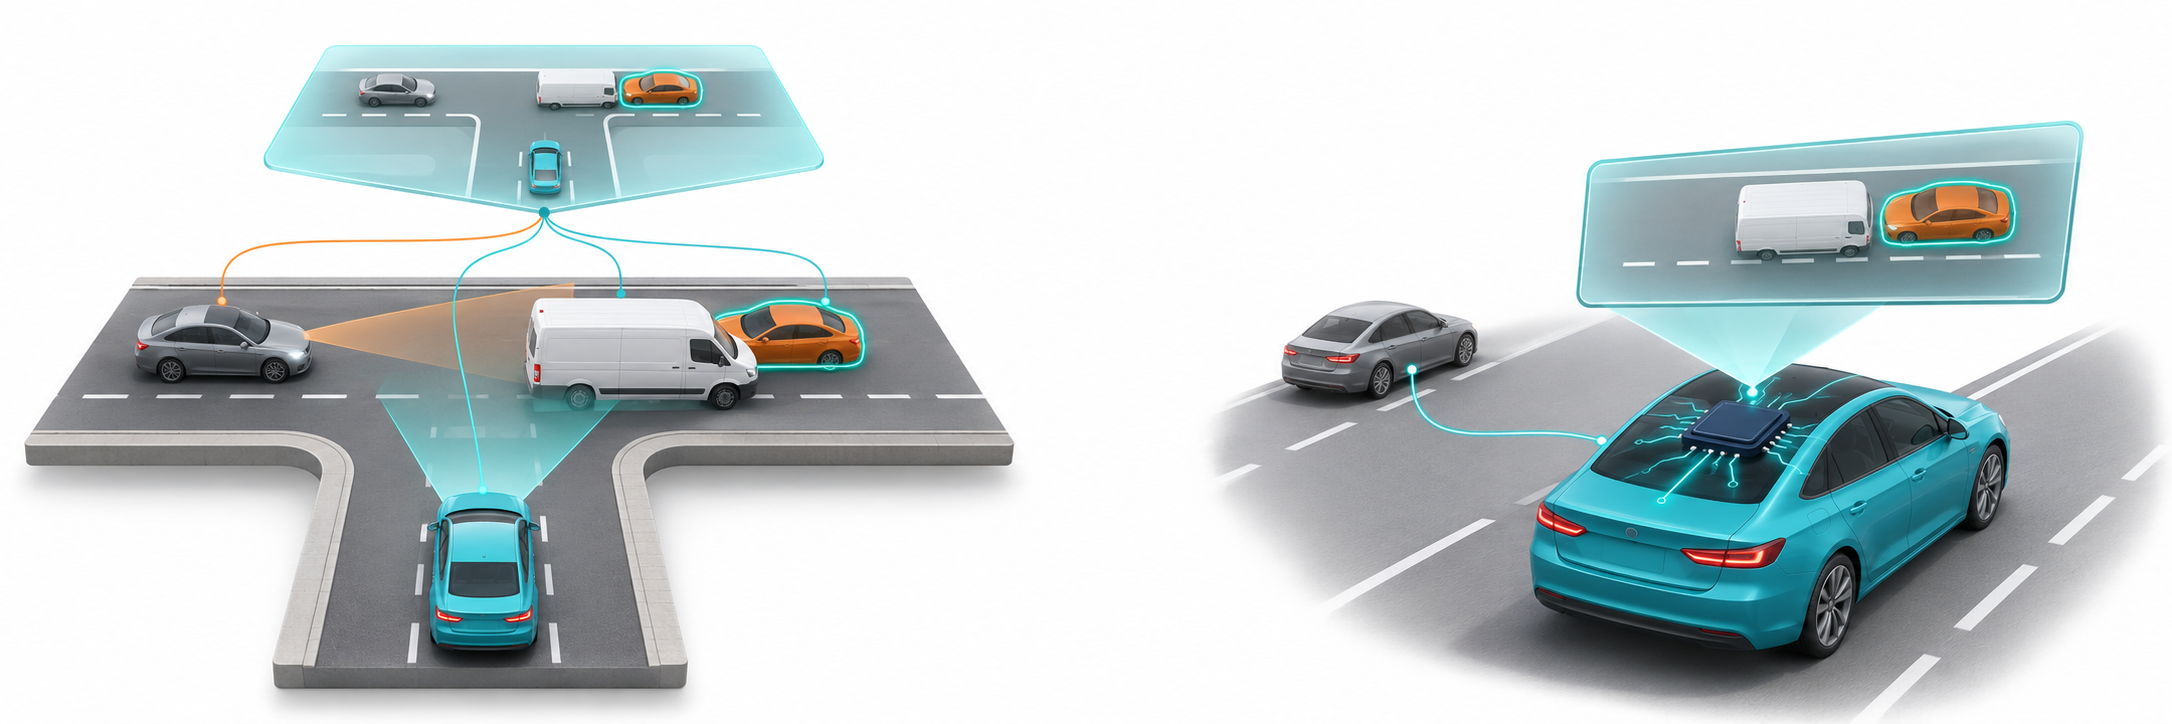
\includegraphics[width=11.1cm]{assets/illustrations/problem/problem-holistic-onboard-imagegen-v2.png}};
    \node[final statement,text width=14.4cm,
      font=\sffamily\fontsize{16}{20}\selectfont] at (7.4,5.28)
      {Can a Holistic Early-Fusion Model Be Compressed\\
      While Preserving Detection Accuracy?};
    \node[final heading] at (4.2,4.40) {Holistic Teacher};
    \node[final heading] at (10.8,4.40) {Collaborative Student};
    \node[visual small,anchor=center] at (4.2,4.00) {Early Fusion};
    \node[visual small,anchor=center] at (10.8,4.00) {DiscoNet};
    \draw[visual arrow,dashed] (6.20,3.70) --
      node[above,align=center,text=MoverNavy,font=\fontsize{9}{11}\selectfont]
        {Distillation\\Training Only} (8.60,3.70);
  \end{VisualCanvas}}
  \SlideSource{Source: AI generated illustrations.}
\end{frame}
